
\documentclass[handout]{beamer}
\usepackage{amsfonts}
\usepackage{amsmath}

\usetheme{Madrid}

\title[ALARI Statistics Course]{ALARI Statistics Course}
\subtitle{Part II}
\author[Claudio Ortelli]{Claudio Ortelli}
\institute[USI]{Universit\`{a} della Svizzera italiana}
\date[29/2010]{April 2010}

\begin{document}
\maketitle


\section{Some special distributions with applications}


\begin{frame}{Some special distributions with applications}{The memoryless property of the exponential distribution}
Le $X\sim Exp(\lambda)$ be the lifetime of a component. Suppose we have observed that it has already been operating 
for $t$ hours.
\begin{itemize}
 \item What is the distribution of the remaining (residual) lifetime $Y=X-t$?
\end{itemize}
Let the conditional probability of $Y \leq y$, given that $X>t$, be denoted by $G_Y(y\rvert t)$. For $y\geq 0$

\begin{eqnarray*}
G_Y(y\rvert t) &=& P(Y \leq y \rvert X>t) = \frac{P(\{Y \leq y \} \textnormal{ and } \{X>t\})}{P(X>t)} \\
&=& \frac{P(\{X \leq y+t \} \textnormal{ and } \{X>t\})}{P(X>t)} = \frac{P(t < X \leq y+t)}{P(X>t)} \\
&=& \frac{exp(-\lambda t)(1-exp(-\lambda y))}{exp(-\lambda t)} = 1-exp(-\lambda y).
\end{eqnarray*}
\end{frame}
 

\begin{frame}{Some special distributions with applications}{The memoryless property of the exponential distribution}
Result:\\
The conditional distribution $G_Y(y\rvert t)$ does not depend on $t$ and is identical to the distribution of $X$, i.e. 
$Exp(\lambda)$.\\
\vspace{1cm}
Interpretation:\\
The distribution of the remaining life does not depend on how long the component has been operating, i.e. the component 
does not age (it is as good as new). Therefore, the exponential distribution is not suited to model components or devices
that gradually deteriorate.  

\end{frame}

\begin{frame}{Some special distributions with applications}{The reliability and failure rate}
Let the random variable $X$ be the lifetime (or time to failure) of a component.
\begin{definition}
 The \textbf{reliability} $R(t)$ of the component is the probability that the component survives until some time $t$, i.e. 
\[
 R(t) = P(X>t) = 1-F_X(t)
\]
$F_X(t)$ is often called the \textbf{unreliability} of the component.
\end{definition}
The conditional probability that the component  \textcolor{red}{does not} survive for an additional interval of duration $x$ 
given that it has survived until time $t$ is equal to
\[
 G_Y(x \rvert t) = \frac{P(t< X \leq t+x)}{P(X>t)} = \frac{F_X(t+x) - F_X(t)}{R(t)}
\]
\end{frame}

\begin{frame}{Some special distributions with applications}{The reliability and failure rate}
\begin{definition}
The instantaneous failure rate $h(t)$ is defined to be
\[
 h(t) = \lim_{x \rightarrow 0} \frac{1}{x} G_Y(x \rvert t) = \lim_{x \rightarrow 0} \frac{F_X(t+x) - F_X(t)}{xR(t)} \ ,
\]
so that
\[
 h(t) = \frac{f_X(t)}{R(t)}.
\]
\end{definition}
Alternate terms for $h(t)$ are \textit{hazard rate}, \textit{force of mortality}, \textit{intensity rate}, 
\textit{conditional failure rate} or \textbf{failure rate}.\\
Interpretation:
\begin{itemize}
 \item $h(t)\Delta t$ represents the conditional probability that a component having survived to age $t$ will 
fail in the interval $(t,t+\Delta t]$.
\end{itemize}
\end{frame}

\begin{frame}{Some special distributions with applications}{The reliability and failure rate}%[allowframebreaks]
\begin{itemize}
 \item $f_X(t) \Delta t$ is the \textit{unconditional} probability while $h(t)\Delta t$ is a conditional probability.
\end{itemize}
Next theorem shows the connection between reliability and failure rate.
\begin{theorem}
 \[
R(t) = \exp\left( - \int_0^t h(x)dx \right)  
 \]
\end{theorem}
\begin{proof}
\[
  \int_0^t h(x)dx  =  \int_0^t \frac{f_X(t)}{R(t)}dx =\int_0^t \frac{-R'(t)}{R(t)}dx = - \ln(R(t))
\]
using the fact that $R'(t)=-f_X(t)$ and the boundary contition $R(0)=1$.
\end{proof}

\end{frame}

\begin{frame}{Some special distributions with applications}{The reliability and failure rate}
 \begin{definition}
  The cumulative hazard is defined to be 
\[
 H(t) = \int_0^t h(x) dx
\]
 \end{definition}
Then, reliability can also be written as $R(t) = \exp(-H(t))$.
\begin{definition}\label{DefConditionalReliability}
The conditional reliability $R_t(y)$ is the probability that the component survives an additional 
interval of duration $y$ given that it has survived until time $t$.
\begin{eqnarray}
 R_t(y) =  \frac{R(t+y)}{R(t)} \label{conditionalReliability}
\end{eqnarray}
 \end{definition}
\end{frame}

\begin{frame}{Some special distributions with applications}{The reliability and failure rate}
Assume a component does not age stochastically, i.e. the survival probability over an additional
time interval $y$ is the same regardless of the age $t$ of the component:
\begin{eqnarray*}
 R_t(y) &=& R_s(y) \textnormal{ \ for all } t,s \geq 0.
\end{eqnarray*}
For $s=0$
\begin{eqnarray*}
 R_t(y) &=& R_0(y) = \frac{R(y)}{R(0)} = R(y),
\end{eqnarray*}
so that
\begin{eqnarray*}
 R(t+y) &=& R(t) R(y).
\end{eqnarray*}
In particular we obtain
\begin{eqnarray*}
 \frac{R(t+y) - R(y)}{t} &=& \frac{(R(t)-1)R(y)}{t}=\frac{(R(t)-R(0))R(y)}{t}.
\end{eqnarray*}
\end{frame}

\begin{frame}{Some special distributions with applications}{The reliability and failure rate}
Taking the limit as $t\rightarrow0$ 
  \begin{eqnarray*}
R'(y) &=& R'(0)R(y) \\
R(y) &=& \exp(yR'(0)) = \exp(-\lambda y)
  \end{eqnarray*}
which shows that the lifetime $X \sim Exp(\lambda)$.\\
If a component has exponential lifetime distribution it follows that
\begin{enumerate}
\item A replacement policy of used components based on the lifetime of the components is useless.
\item In estimating mean life and reliability the age of the observed components are of no concern.
The number of hours of observed live and the number of observed failures are of interest. 
\end{enumerate}

\end{frame}

\begin{frame}{Some special distributions with applications}{The reliability and failure rate}
\begin{definition}
Increasing (decreasing) failure rate distribution\\
Let $X$ be the lifetime of a component and $F_X(t)$ the corresponding distribution function.
If its failure rate $h(t)$ is an increasing (decreasing) function of $t$ for $t \geq 0$ then $F_X$ is an Increasing (Decreasing) Failure 
Rate distribution: IFR (DFR) distribution.
\end{definition}

\end{frame}
\begin{frame}{Some special distributions with applications}{The reliability and failure rate}
 The behavior of the failure rate $h(t)$ as a function of age is known as the \textit{mortality curve}, 
\textit{hazard function}, \textit{life characteristic} or \textit{lambda characteristic}.
\begin{center}
 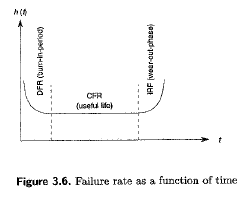
\includegraphics[width=110pt,keepaspectratio=true]{./Figura3_6.png}
 % Figura3.6: 336x256 pixel, 90dpi, 9.48x7.23 cm, bb=0 0 269 205
\end{center}

\end{frame}


\begin{frame}{Some special distributions with applications}{Hypoexponential Distribution}
The hypoexponential distribution is used to model processes that can be divided into sequential 
phases such that the time the process spends in each phase is independent and exponentially distributed.
\begin{itemize}
 \item Service times for input-output operations in a computer system often follow this distribution.
\end{itemize}
A two stage hypoexponential random variable $X \sim Hypo(\lambda_1,\lambda_2)$ has pdf and distribution function equal to
 \begin{eqnarray*}
f(t) &=& \frac{\lambda_1 \lambda_2}{\lambda_2 - \lambda_1} ( \exp(- \lambda_1 t) - \exp(\lambda_2 t) ), \ \ t> 0 \\ 
F(t) &=& 1 - \frac{\lambda_2}{\lambda_2 - \lambda_1} \exp(- \lambda_1 t) + \frac{\lambda_1}{\lambda_2 - \lambda_1}\exp(- \lambda_2 t)
 \end{eqnarray*}

\end{frame}

\begin{frame}{Some special distributions with applications}{Erlang Distribution}
When $r$ sequential phases have identical exponential distribution the resulting density is known as
$r-$stage Erlang and is given by

 \begin{eqnarray*}
f(t) &=& \frac{\lambda ^r t ^{r-1}  \exp(-\lambda t)}{(r-1)!}  \textnormal{ with } t>0, \ \lambda > 0, \ r=1,2,\dots \\ 
F(t) &=& 1 - \sum_{k=0}^{r-1} \frac{(\lambda t)^k}{k!} \exp(- \lambda t) \textnormal{ with } t \geq 0, \ \lambda > 0, \ r=1,2,\dots 
 \end{eqnarray*}

\end{frame}


\begin{frame}{Some special distributions with applications}{Hyperexponential Distribution}
Suppose that a process consists of alternate phases, i.e. during any single experiment the process 
experiences one and only one of the many alternate phases, and thes phases have exponential distributions.
The overall distribution is then hyperexponential with density and distribution functions given by

 \begin{eqnarray*}
f(t) &=& \sum_{i=1}^k \alpha_i \lambda_i \exp(-\lambda_i t)  \textnormal{ with } t>0, \ \lambda_i > 0, \ \sum_{i=1}^{k}\alpha_i=1\\ 
F(t) &=& \sum _i \alpha_i (1-\exp(\lambda_i t)) \ \ t \geq 0
 \end{eqnarray*}

\end{frame}


\begin{frame}{Some special distributions with applications}{Weibull Distribution}
The Weibull distribution is the most widely used parametric family of failure distributions. It has been used to describe
\begin{itemize}
 \item fatigue failure
 \item electronic component failure
 \item ballbearing failure
\end{itemize}
The reason is that by a proper choice of the shape parameter $\alpha$ we can obtain an IFR, DFR or constant failure rate 
distribution. The corresponding density and distribution functions are given by

 \begin{eqnarray*}
f(t) &=& \lambda \alpha t^{\alpha -1} \exp(-\lambda t ^\alpha)\\ 
F(t) &=&  1 - \exp(-\lambda t ^\alpha)
 \end{eqnarray*}
where $t \geq 0$, $\lambda > 0$ and $\alpha > 0$.
\end{frame}

\begin{frame}{Some special distributions with applications}{Pareto Distribution}
 The Pareto (also knonw as double-exponential, hyperbolic or power-law) distribution has been used 
to model 
\begin{itemize}
\item the amount of CPU time consumed by an arbitrary process
\item the Web file size on the Internet servers
\item the thinking time of the web browser
\item the number of data bytes in FTP bursts
\item the access frequency of Web traffic 
\end{itemize}
The density and distributions functions are given by
 \begin{eqnarray*}
f(x) &=& \alpha k^{\alpha} x^{-\alpha -1} \ \ x \geq k, \ k>0, \ \alpha > 0\\ 
F(x) &=& \left\{ \begin{array}{l l}
            1 - \left( \frac{k}{x} \right) ^\alpha & \ x \geq k \\
            0 & x < k    
           \end{array} \right. 
 \end{eqnarray*}
\end{frame}



\end{document}
